\section{Hybrid cavity}

The third design simulated was a hybrid cavity consisting of a right-handed chiral gain medium placed between two left-handed chiral media acting as reflectors for left-circularly polarised light reflectors. The design is schematised in figure \ref{fig:hybrid}.

The lasing action of the cavity is simulated using the same method as before with the parameters given in table \ref{tab:hybrid_cavity:simulation}. Losses were added in the reflectors because otherwise zero-gain modes can be found. This makes sense mathematically because that means such modes are able to perform a round-trip in the cavity without being altered, but does not correspond to any physical reality as mirrors are necessary slightly lossy. Figure \ref{fig:hybrid_cavity:mycwt_surf} show the lasing coefficient found with approximate theory (the result with exact theory was very close and thus is not shown). The corresponding output modes are then calculated for both method, and the intensity distributions are plotted in figure \ref{fig:hybrid_cavity:modes}.

The first thing to be noted is that this geometry allows producing very pure left or right circularly polarised modes. The second thing is that mode 1 requires left-handed light coming from the outside of the cavity. This is attributed to an imprecise localisation of this mode. The three displayed modes allow illustrating the dynamics at play in the cavity leading to the two possible output handedness. First, for left-handed output polarisations, light is not reflected by right-handed medium and travels in left-handed media, leading to chirality-preserving reflections schematised in figure \ref{fig:hybrid:mechanism_lh}. Then, for right-handed modes, the cavity acts as a simple cavity\cite{topf_modes_2014} with index-matched media at the interfaces, thus providing pure right-handed circularly polarised output as there are no Fabry-Pérot modes. This dynamic is  shown in figure \ref{fig:hybrid:mechanism_rh} and explains mode 3 in figure \ref{fig:hybrid_cavity:modes}.


\begin{table}
	\centering
	\begin{tabulary}{\linewidth}{LCC}
		\hline
		\hline
		Structural period of the chiral medium & $L_p$ & 300 nm \\
		Length of the left-handed chiral media & $L_L$ & $40\times L_p$ \\
		Length of the right-handed chiral media & $L_R$ & $20\times L_p$ \\
		Refractive index of the surrounding media & $n_1=n_2$ & 1 \\
		Average refractive index of the chiral media (Re) & $\Re{\bar{n}_{L,R}}$ & 1.7690 \\
		Average refractive index of the left-handed chiral media (Im) & $\Im{\bar{n}_L}$ & 0.02 \\
		Detuning range & $\mathrm{Re}(\delta k L_R / 2)$ & $[0,6]$ \\
		Gain range & $-\mathrm{Im}(\delta k L_R / 2)$ & $[0,3]$ \\
		Coupling constant & $\kappa_{L,R}$ & $4/L_{L,R}$\\
		\hline
		\hline
	\end{tabulary}
	\caption[Parameters for the cavity with a defect]{Parameters used for simulation.}
	\label{tab:hybrid_cavity:simulation}
\end{table}


\begin{figure}
	\centering
	\begin{subfigure}{0.48\linewidth}
		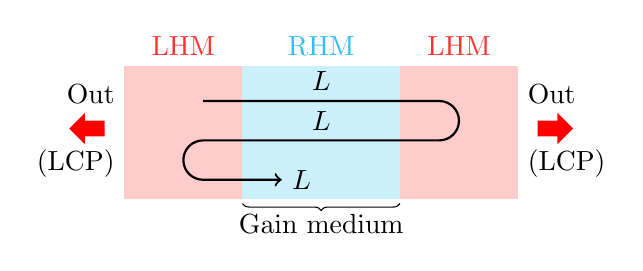
\begin{tikzpicture}
		\fill[red!20] (-1.5,1.2) -- (0,1.2) -- (0,-0.5) -- (-1.5,-0.5) -- cycle;
		\fill[red!20] (2,1.2) -- (3.5,1.2) -- (3.5,-0.5) -- (2,-0.5) -- cycle;
		\fill[cyan!20] (0,1.2) -- (2,1.2) -- (2,-0.5) -- (0,-0.5) -- cycle;
		\draw[red!80] (-0.75,1.2)node [above] {LHM} ;
		\draw[red!80] (2.75,1.2)node [above] {LHM} ;
		\draw[cyan!80] (1,1.2)node [above] {RHM} ;
		
		\draw[->, thick] (-0.5,0.75) -- node[above] {$L$} (2.5,0.75) arc  (90:-90:0.25) -- node[above] {$L$} (-0.5,0.25) arc (90:270:0.25) -- (0.5,-0.25) node[right] {$L$};
		\draw[decoration={brace,mirror,raise=1.5pt},decorate] (0,-0.5) -- node[below=2pt] {Gain medium} (2,-0.5);
		
		\fill[red] (3.75,0.5) -- (4,0.5) -- (4,0.6) -- (4.2,0.4) -- (4,0.2) -- (4,0.3) -- (3.75,0.3) -- cycle;
		\node[above right] at (3.5,0.6) {Out};
		\node[below right] at (3.5,0.25) {(LCP)};			
		
		\fill[red] (-1.75,0.5) -- (-2,0.5) -- (-2,0.6) -- (-2.2,0.4) -- (-2,0.2) -- (-2,0.3) -- (-1.75,0.3) -- cycle;
		\node[above left] at (-1.5,0.6) {Out};
		\node[below left] at (-1.5,0.25) {(LCP)};
		
		\end{tikzpicture}
		\caption{}
		\label{fig:hybrid:mechanism_lh}
	\end{subfigure}
	\begin{subfigure}{0.48\linewidth}
		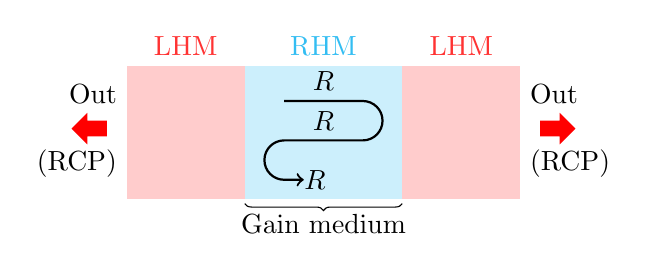
\begin{tikzpicture}
		\fill[red!20] (-1.5,1.2) -- (0,1.2) -- (0,-0.5) -- (-1.5,-0.5) -- cycle;
		\fill[red!20] (2,1.2) -- (3.5,1.2) -- (3.5,-0.5) -- (2,-0.5) -- cycle;
		\fill[cyan!20] (0,1.2) -- (2,1.2) -- (2,-0.5) -- (0,-0.5) -- cycle;
		\draw[red!80] (-0.75,1.2)node [above] {LHM} ;
		\draw[red!80] (2.75,1.2)node [above] {LHM} ;
		\draw[cyan!80] (1,1.2)node [above] {RHM} ;
		
		\draw[->, thick] (0.5,0.75) -- node[above] {$R$} (1.5,0.75) arc  (90:-90:0.25) -- node[above] {$R$} (0.5,0.25) arc (90:270:0.25) -- node[right] {$R$} (0.75,-0.25);
		\draw[decoration={brace,mirror,raise=1.5pt},decorate] (0,-0.5) -- node[below=2pt] {Gain medium} (2,-0.5);
		
		\fill[red] (3.75,0.5) -- (4,0.5) -- (4,0.6) -- (4.2,0.4) -- (4,0.2) -- (4,0.3) -- (3.75,0.3) -- cycle;
		\node[above right] at (3.5,0.6) {Out};
		\node[below right] at (3.5,0.25) {(RCP)};
		
		
		\fill[red] (-1.75,0.5) -- (-2,0.5) -- (-2,0.6) -- (-2.2,0.4) -- (-2,0.2) -- (-2,0.3) -- (-1.75,0.3) -- cycle;
		\node[above left] at (-1.5,0.6) {Out};
		\node[below left] at (-1.5,0.25) {(RCP)};
		
		\end{tikzpicture}
		\caption{}
		\label{fig:hybrid:mechanism_rh}
	\end{subfigure}
	\caption[Mechanisms leading to laser action in an hybrid cavity]{Mechanisms leading to laser action in an hybrid cavity. \ref{fig:hybrid:mechanism_lh} Reflections of left-handed light on the reflectors. \ref{fig:hybrid:mechanism_rh} Reflections of right-handed light inside the gain medium.}
	
\end{figure}

\begin{figure}
	\centering
	\begin{subfigure}{0.49\textwidth}
		\begin{subfigure}{\textwidth}
			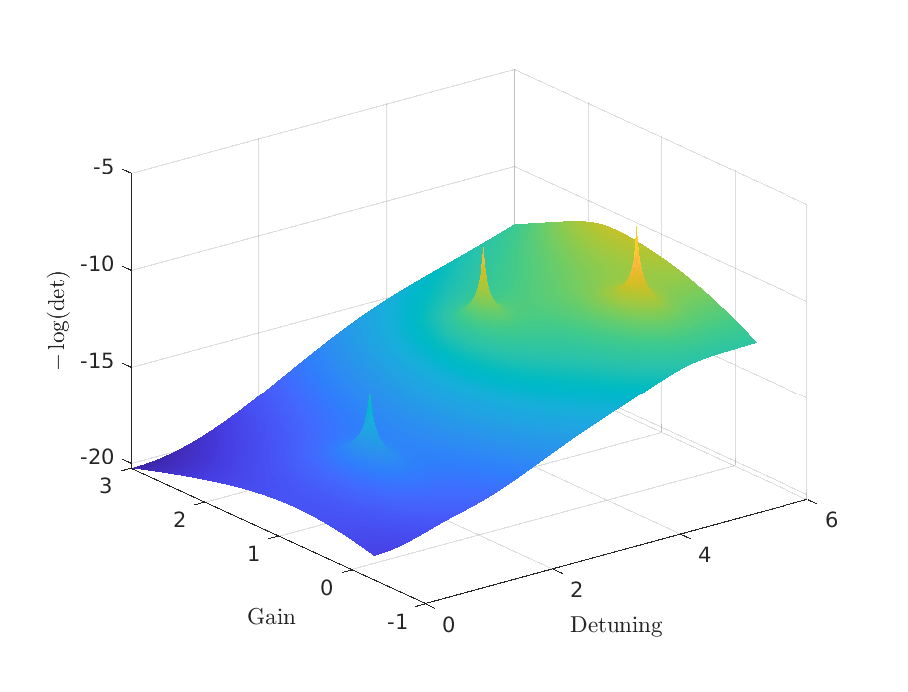
\includegraphics[width=\textwidth]{plots/hybrid/surface}
			\caption{}
			\label{fig:hybrid_cavity:mycwt_surf}
		\end{subfigure}	
		\begin{subfigure}{\textwidth}
			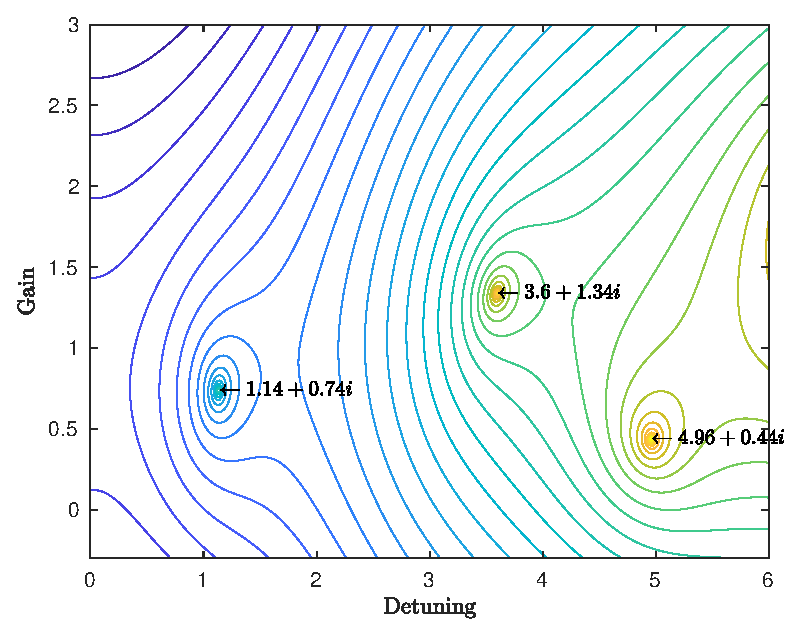
\includegraphics[width=\textwidth]{plots/hybrid/contour}
			\caption{}
			\label{fig:hybrid_cavity:mycwt_contour}
		\end{subfigure}
	\end{subfigure}
	\begin{subfigure}{0.49\textwidth}
		\begin{subfigure}{\textwidth}
			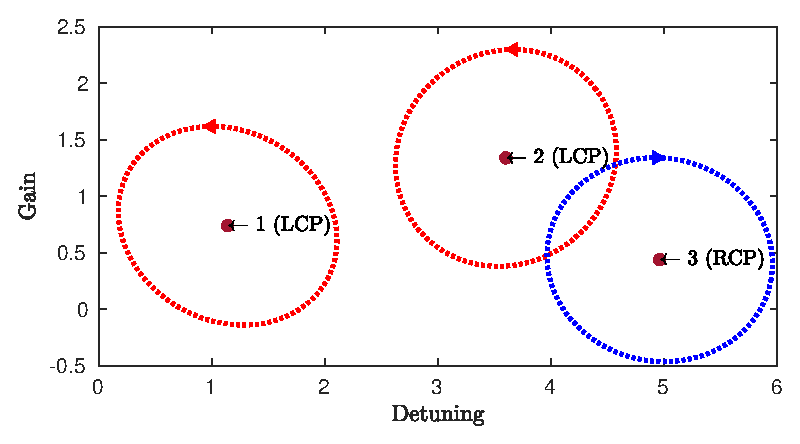
\includegraphics[width=\textwidth]{plots/hybrid/modes_found}
			\caption{Developed CWT}
			\label{fig:hybrid_cavity:modes_found}
		\end{subfigure}
		\begin{subfigure}{\textwidth}
			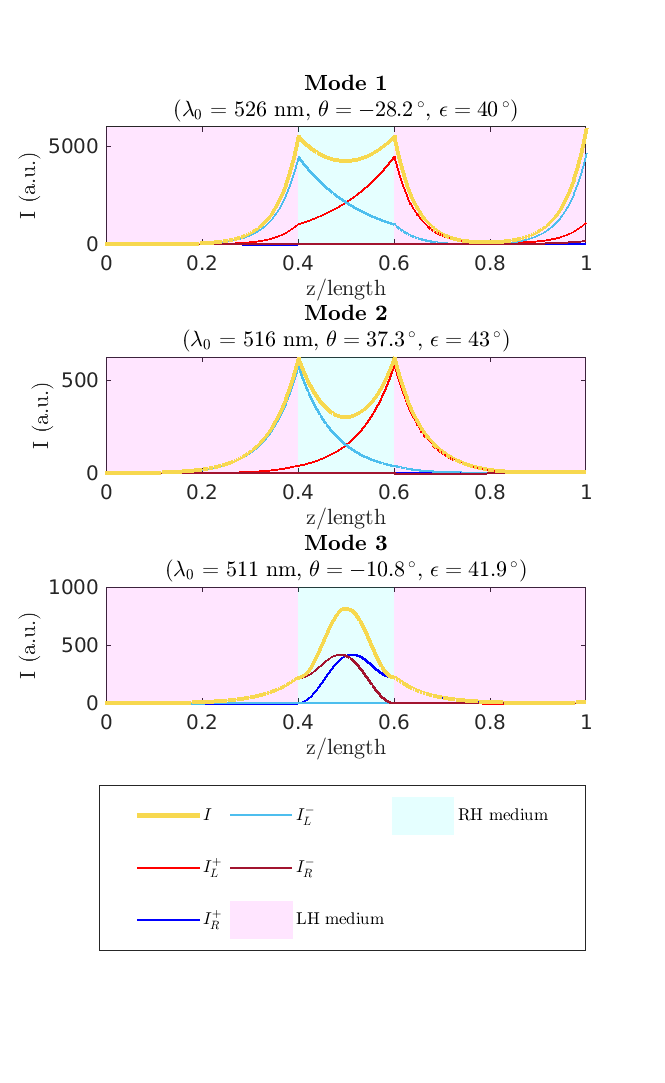
\includegraphics[width=\textwidth]{plots/hybrid/intensity_distribution}
			\caption{}
			\label{fig:hybrid_cavity:intensity_distribution}
		\end{subfigure}
	\end{subfigure}
	\caption[Analysis of hybrid cavity]{Analysis of hybrid cavity. \ref{fig:hybrid_cavity:mycwt_surf} shows the logarithm of the invert of the determinant of $\bm{M_{22}}$. \ref{fig:hybrid_cavity:mycwt_contour} is the corresponding contour plot where the lasing modes have been identified. \ref{fig:hybrid_cavity:modes_found} Labeled modes found with the developed CWT and corresponding output ellipses in medium 1. \ref{fig:hybrid_cavity:intensity_distribution} Intensity distribution in the cavity for the modes in \ref{fig:hybrid_cavity:modes_found}. The results yielded by exact theory are similar and are presented in figure \ref{fig:hybrid_intensity_appendix} in appendix \ref{chap:intensities}.}
	\label{fig:hybrid_cavity:modes}
\end{figure}

\subsection{Conclusion on hybrid cavity}

The hybrid cavity geometry solves the issue of impurities present in the output of a simple cavity and a defect cavity. This is because the hybrid geometry simplifies the dynamics of reflections in the cavity, removing the chirality-reversing reflections due to unmatched index interfaces. The left-handed modes require higher gain, because of the losses in left-handed media where the reflections occur.